\documentclass[tikz]{standalone}
\begin{document}

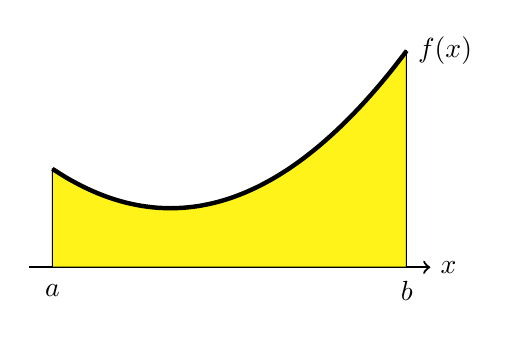
\begin{tikzpicture}[xscale=3,yscale=3.0]
  \draw[thick,->] (-0.6,0) -- (1.1,0) node[right] {$x$};
  \node at (-0.5, -0.1){$a$};
  \node at (1, -0.1) {$b$};
  \draw[fill=yellow!90] (-0.5,0) -- plot[smooth, samples=100, domain=-0.5:1 ] (\x,\x*\x/1.5 + 0.25) |- (-0.5,0);
  \draw[ultra thick,domain=-0.5:1,smooth,variable=\x,black] plot (\x,\x*\x/1.5 + 0.25) node[right]{$f(x)$};
\end{tikzpicture}
~~~
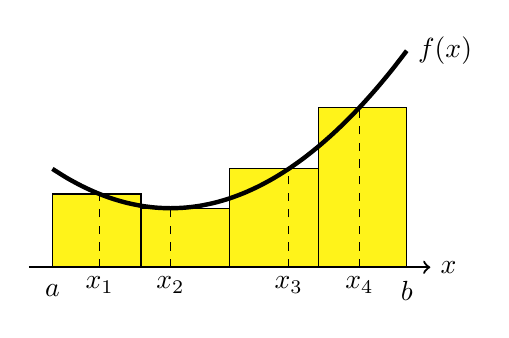
\begin{tikzpicture}[xscale=3,yscale=3.0]
  \node at (-0.5, -0.1){$a$};
  \node at (1, -0.1) {$b$};

  \draw[fill=yellow!90] (-0.5,0) rectangle ++(0.375,{(-0.3)^2 / 1.5 + 0.25});
  \draw [dashed] (-0.3,0) node[below] {$x_1$} -- (-0.3,{(-0.3)^2 / 1.5 + 0.25});

  \draw[fill=yellow!90] (-0.125,0) rectangle ++(0.375,{(0.0)^2 / 1.5 + 0.25});
  \draw [dashed] (0.0,0) node[below] {$x_2$} -- (0.0,{(0.0)^2 / 1.5 + 0.25});
        
  \draw[fill=yellow!90] (0.250,0) rectangle ++(0.375,{(0.5)^2 / 1.5 + 0.25});
  \draw [dashed] (0.5,0) node[below] {$x_3$} -- (0.5,{(0.5)^2 / 1.5 + 0.25});

  \draw[fill=yellow!90] (0.625,0) rectangle ++(0.375,{(0.8)^2 / 1.5 + 0.25});
  \draw [dashed] (0.8,0) node[below] {$x_4$} -- (0.8,{(0.8)^2 / 1.5 + 0.25});
        
  \draw[thick,->] (-0.6,0) -- (1.1,0) node[right] {$x$};
  \draw[ultra thick,domain=-0.5:1,smooth,variable=\x,black] plot (\x,\x*\x/1.5 + 0.25) node[right]{$f(x)$};

\end{tikzpicture}
\end{document} 
